\section{Architektur}
\label{sec:arch}

Zu Anfang ist es sinnvoll, die Architektur des Systems festzulegen.
Diese bestimmt, welche Komponenten und Microservices entwickelt und verbunden werden müssen.
Der erste Schritt dabei ist es, die Aufgaben aufzuteilen, die das System erfüllen soll und dann auf Microservices verteilt werden.
Die weitere Entwicklung des Systems stützt sich dann auf die fertige Architektur.

Eine erste und offensichtliche Aufteilung gibt bei den benötigten Arbeitsschritten Laden der Daten, Deltaberechnung und Speichern der Daten.
Da diese aber ein zusammenhängender Prozess sind, der in ein Job in Spark ausgeführt wird, sollte hier auch keine Aufteilung geschehen.
Besser ist die Betrachtung verschiedener Funktionen.
Hier findet man die API, das kontinuierliche Ausführen und die Ingestion mit Spark der Daten als gut trennbare Teile.

Bei der \textbf{API} handelt es sich um den Service für die Interaktion mit dem Data-Lake-System.
Durch die Anforderungen ist bereits festgelegt, dass dieser ein Web-Server mit einer REST-Schnittstelle ist.
Es geht zwar in dieser Arbeit nur um die Ingestion, aber der API-Service sollte Schnittstellen zu allen Funktionen des Data-Lake-Systems enthalten.

Die \textbf{Ingestion} ist dafür zuständig, die Datenquellen zu verarbeiten und den kompletten Prozess vom Laden bis zum Speichern der Daten in \textit{Apache Spark} auszuführen.
Die Ausführung soll für eine Datenquelle nur einmal gleichzeitig aber parallel für unterschiedliche laufen.

Bei einer zeitgesteuerten oder Datenstrom-Ingestion muss die \textbf{kontinuierliche Ausführung} sichergestellt werden.
Für alle Datenquellen muss regelmäßig geprüft werden, ob für diese gerade eine Ingestion ausgeführt wird und ausgeführt werden sollten.
Falls keine ausgeführt wird aber sollte, wird die Ingestion für diese Datenquelle gestartet.

Neben diesen Mircoservices wird noch ein Nachrichtensystem benötigt.
Das Nachrichtensystem stellt die Kommunikation zwischen den Microservices dar.
Hier ist es wichtig, dass es einem Sender möglich ist, Nachrichten an einen oder auch an mehrere Empfänger zu senden.
So soll sichergestellt werden, dass bestehende Microservices einfach repliziert und neue eingefügt werden können.

Es werden zwei Speicher benötigt.
Eine Datenbank, die ausschließlich prozeduale Daten enthält.
Das sind alle Daten, die für die Funktion des Systems notwenig sind.
Und den Speicher für die Ablage aller aufgenommen Daten.

\begin{figure}
    \centering
    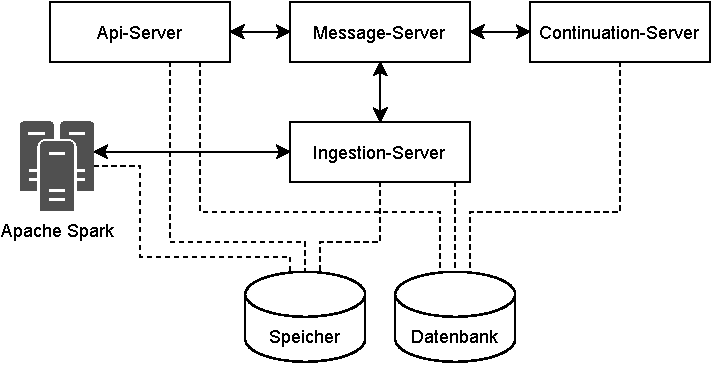
\includegraphics{Grafiken/Entwicklung-System-Architektur.pdf}
    \caption{System Architektur der Ingestion}
    \label{fig:system-architektur}
\end{figure}
